\documentclass[hidelinks,12pt]{article}
\usepackage[left=0.25cm,top=1cm,right=0.25cm,bottom=1cm]{geometry}
%\usepackage[landscape]{geometry}
\textwidth = 20cm
\hoffset = -1cm
\usepackage[utf8]{inputenc}
\usepackage[spanish,es-tabla]{babel}
\usepackage[autostyle,spanish=mexican]{csquotes}
\usepackage[tbtags]{amsmath}
\usepackage{nccmath}
\usepackage{amsthm}
\usepackage{amssymb}
\usepackage{mathrsfs}
\usepackage{graphicx}
\usepackage{subfig}
\usepackage{standalone}
\usepackage[outdir=./Imagenes/]{epstopdf}
\usepackage{siunitx}
\usepackage{physics}
\usepackage{color}
\usepackage{float}
\usepackage{hyperref}
\usepackage{multicol}
%\usepackage{milista}
\usepackage{anyfontsize}
\usepackage{anysize}
%\usepackage{enumerate}
\usepackage[shortlabels]{enumitem}
\usepackage{capt-of}
\usepackage{bm}
\usepackage{relsize}
\usepackage{placeins}
\usepackage{empheq}
\usepackage{cancel}
\usepackage{wrapfig}
\usepackage[flushleft]{threeparttable}
\usepackage{makecell}
\usepackage{fancyhdr}
\usepackage{tikz}
\usepackage{bigints}
\usepackage{scalerel}
\usepackage{pgfplots}
\usepackage{pdflscape}
\pgfplotsset{compat=1.16}
\spanishdecimal{.}
\renewcommand{\baselinestretch}{1.5} 
\renewcommand\labelenumii{\theenumi.{\arabic{enumii}})}
\newcommand{\ptilde}[1]{\ensuremath{{#1}^{\prime}}}
\newcommand{\stilde}[1]{\ensuremath{{#1}^{\prime \prime}}}
\newcommand{\ttilde}[1]{\ensuremath{{#1}^{\prime \prime \prime}}}
\newcommand{\ntilde}[2]{\ensuremath{{#1}^{(#2)}}}

\newtheorem{defi}{{\it Definición}}[section]
\newtheorem{teo}{{\it Teorema}}[section]
\newtheorem{ejemplo}{{\it Ejemplo}}[section]
\newtheorem{propiedad}{{\it Propiedad}}[section]
\newtheorem{lema}{{\it Lema}}[section]
\newtheorem{cor}{Corolario}
\newtheorem{ejer}{Ejercicio}[section]

\newlist{milista}{enumerate}{2}
\setlist[milista,1]{label=\arabic*)}
\setlist[milista,2]{label=\arabic{milistai}.\arabic*)}
\newlength{\depthofsumsign}
\setlength{\depthofsumsign}{\depthof{$\sum$}}
\newcommand{\nsum}[1][1.4]{% only for \displaystyle
    \mathop{%
        \raisebox
            {-#1\depthofsumsign+1\depthofsumsign}
            {\scalebox
                {#1}
                {$\displaystyle\sum$}%
            }
    }
}
\def\scaleint#1{\vcenter{\hbox{\scaleto[3ex]{\displaystyle\int}{#1}}}}
\def\bs{\mkern-12mu}


%\usepackage{showframe}
\title{Ejercicios con la Transformadas de Laplace \\ \large {Tema 6 - Transformadas integrales} \vspace{-3ex}}
\author{M. en C. Gustavo Contreras Mayén}
\date{ }
\begin{document}
\vspace{-4cm}
\maketitle
\fontsize{14}{14}\selectfont
\tableofcontents
\newpage

\section{Ejercicios.}

\subsection{Problema con valores iniciales.}
Resolver el siguiente problema con valores iniciales:
\begin{align*}
\stilde{x} - \ptilde{x} - 6 \, x = 2, \hspace{1cm} x(0)=2, \hspace{0.4cm} x^{\prime}(0) = -1
\end{align*}
Con los valores iniciales dados, la transformada de Laplace de la derivada de primer y segundo orden, nos conducen a que
\begin{align*}
L \big[x^{\prime}(t)\big] = s \, L \big[x(t)\big] - x(0) =  s \, X(s) - 2
\end{align*}
y
\begin{align*}
L \big[\stilde{x}(t)\big] = s^{2} \, L \big[x(t)\big] - s \, x(0) - \stilde{x} (0) =  s^{2} \, X(s) - 2 \, s + 1
\end{align*}
donde $X(s)$ representa la transformada de Laplace de la función (desconocida) $x(t)$. De esta manera, la ecuación transformada es
\begin{align*}
\big[ s^{2} \, X(s) - 2 \, s + 1 \big] - \big[ s \, X(s) - 2 \big] - 6 \big[X(s)\big] = 0
\end{align*}
la cual se simplifica rápidamente en
\begin{align*}
(s^{2} - s - 6) \, X(s) - 2 \, s + 3 = 0
\end{align*}
por tanto
\begin{align*}
X(s) = \dfrac{2 \, s - 3}{s^{2} - s - 6} = \dfrac{2 \, s - 3}{(s-3)(s+2)}
\end{align*}
Por el método de fracciones parciales (del cálculo integral), existen constantes $A$ y $B$ tales que
\begin{align*}
\dfrac{2 \, s - 3}{(s-3)(s+2)} =  \dfrac{A}{(s - 3)} + \dfrac{B}{(s+2)}
\end{align*}
y al multiplicar ambos lados de esta ecuación por $(s-3)(s+2)$, se llega a la identidad
\begin{align*}
2 \, s - 3 = A (s + 2) +  B (s - 3)
\end{align*}
Si sustituimos $s = 3$, encontramos que $A = \dfrac{3}{5}$, la sustitución de $s = -2$ muestra que $B = \dfrac{7}{5}$, así tenemos que
\begin{align*}
X(s) = L \big[x(t)\big]  = \dfrac{\frac{3}{5}}{s - 3} + \dfrac{\frac{7}{5}}{s + 2}
\end{align*}
Como la transformada inversa de Laplace:
\begin{align*}
L^{-1} \bigg[\dfrac{1}{(s - a)} \bigg] = e^{a t}
\end{align*}
se sigue que
\begin{align*}
x(t) = \dfrac{3}{5} \, e^{3t} + \dfrac{7}{5} \, e^{-2t}
\end{align*}
es la solución del problema original con valores iniciales. 
\par
Nótese que se encontró primero la solución general de la ecuación diferencial. El método de la transformada de Laplace proporciona directamente la solución particular deseada considerando automáticamente las condiciones iniciales dadas.

\subsection{Sistema masa resorte.}

Resolver el siguiente problema con valores iniciales:
\begin{align*}
\stilde{x} + 4 \, x =  \sin 3 \, t, \hspace{1.5cm} x(0) = \ptilde{x}(0) = 0
\end{align*}
Un problema de este tipo surge en el movimiento de un sistema masa-resorte con una fuerza externa, como se muestra en la figura (\ref{fig:figura_07_02_02}).
\begin{figure}[H]
    \centering
    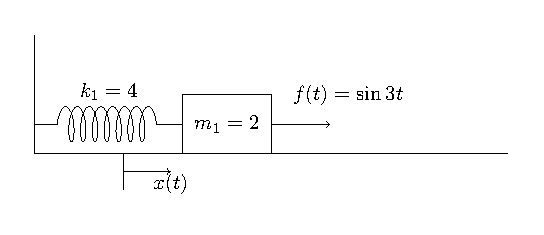
\includegraphics[scale=1.3]{Imagenes/sist_masa_resorte.eps}
    \caption{Sistema masa-resorte que satisface el problema con valores iniciales.}
    \label{fig:figura_07_02_02}
\end{figure}
Debido a que ambas condiciones son cero, la transformada de Laplace de la segunda derivada de $x(t)$, nos devuelve $L \big[\stilde{x} (t)\big] = s^{2} \, X(s) $. La transformada de $\sin 3 \, t$ se obtiene de tablas y de esta manera se encuentra la ecuación transformada:
\begin{align*}
s^{2} \, X(s) + 4 \, X(s) = \dfrac{3}{s^{2} + 9}
\end{align*}
Por tanto
\begin{align*}
X(s) = \dfrac{3}{(s^{2} + 4)(s^{2} + 9)}
\end{align*}
Ocupando el método de fracciones parciales resulta en
\begin{align*}
\dfrac{3}{(s^{2} + 4)(s^{2} + 9)} = \dfrac{A \, s + B}{s^{2} + 4} + \dfrac{C \, s +D}{s^{2} + 9}
\end{align*}
El \enquote{método seguro} para resolver las fracciones consistiría en multiplicar ambos lados de la ecuación por el denominador común, y luego agrupar los coeficientes de iguales potencias de $s$ del lado derecho. Igualando coeficientes de iguales potencias de los dos lados de la ecuación resultante se llega a cuatro ecuaciones lineales que pueden resolverse para obtener $A$, $B$, $C$ y $D$.
\par
Sin embargo, aquí puede anticiparse que $A = C = 0$ debido a que ni el numerador ni el denominador del lado izquierdo involucran alguna potencia impar de $s$, mientras que algún valor diferente de cero le corresponde a los términos de grado impar del lado derecho. De esta manera, $A$ y $C$ se reemplazan por cero antes de resolver las fracciones. El resultado es la identidad
\begin{align*}
3 = B \, (s^{2} + 9) + D \, (s^{2} + 4) =  (B + D) \, s^{2} + (9 \, B + 4 \, D)
\end{align*}
Cuando se igualan coeficientes de iguales potencias de $s$ se obtienen las ecuaciones lineales
\begin{align*}
B + D &= 0 \\
9 \, B + 4 \, D &= 3
\end{align*}
las cuales se resuelven fácilmente para $B = \dfrac{3}{5}$ y $D = - \dfrac{3}{5}$, así
\begin{align*}
X(s) = L \big[x(t)\big] = \dfrac{3}{10} \; \dfrac{2}{s^{2} + 4} \; - \dfrac{1}{5} \; \dfrac{3}{s^{2} + 9}
\end{align*}
Dado que 
\begin{align*}
L \big[ \sin 2 \, t \big] = \dfrac{2}{s^{2} + 4} \\[0.5em]
L \big[ \sin 3 \, t \big] = \dfrac{3}{s^{2} + 9}
\end{align*}
se concluye que
\begin{align*}
x(t) = \dfrac{3}{10} \, \sin 2 \, t - \dfrac{1}{5} \, \sin 3 \, t
\end{align*}
La figura (\ref{fig:figura_07_02_03}) muestra la gráfica de la función de posición de la masa de período $2 \, \pi$. Nótese que una vez más que el método de la transformada de Laplace proporciona la solución directamente sin necesidad de obtener primero la función complementaria y una solución particular de la ecuación diferencial no homogénea original. De esta manera, las ecuaciones no homogéneas se resuelven exactamente igual que las ecuaciones homogéneas.
\begin{figure}[H]
    \centering
    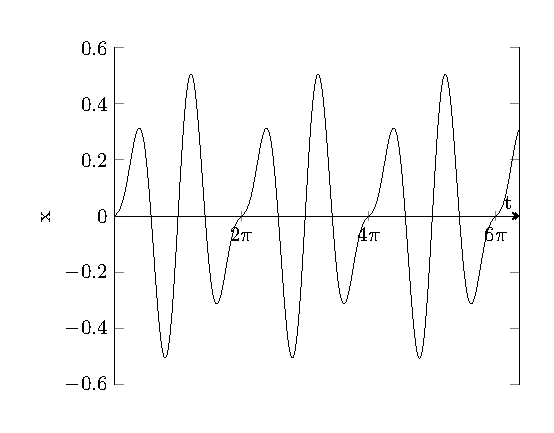
\includegraphics[scale=1.3]{Imagenes/sist_masa_resorte_plot.eps}
    \caption{Función de la posición $x(t)$ del sistema masa-resorte.}
    \label{fig:figura_07_02_03}
\end{figure}

\section{Sistemas lineales.}

La transformada de Laplace se utiliza con frecuencia en problemas para resolver sistemas lineales donde todos los coeficientes son constantes. Cuando se especifican las condiciones iniciales, la transformada de Laplace reduce este sistema lineal de ecuaciones diferenciales a un sistema lineal de ecuaciones algebraicas, donde las incógnitas son las transformadas de las funciones solución. Como se ilustra en el siguiente ejemplo, la técnica para un sistema es esencialmente la misma que para una ecuación diferencial con coeficientes constantes.
\subsection{Sistema mecánico con dos masas.}
Resolver el sistema:
\begin{align}
\begin{aligned}
2 \, \stilde{x} &=  - 6 \, x + 2 \, y \\[0.5em]
\stilde{y} &= 2 \, x - 2 \, y + 40 \sin 3 \, t
\end{aligned}
\label{eq:ecuacion_008}
\end{align}
sujeto a las condiciones iniciales
\begin{align}
x(0) = \ptilde{x} (0) = y(0) = \stilde{y} (0) = 0
\label{eq:ecuacion_009}
\end{align}
De esta manera, la fuerza $f(t) = 40 \sin 3 \, t$ se aplica a la segunda masa de la figura (\ref{fig:figura_005}), iniciando en el tiempo $t=0$ cuando el sistema está en reposo en su posición de equilibrio.
\begin{figure}[H]
    \centering
    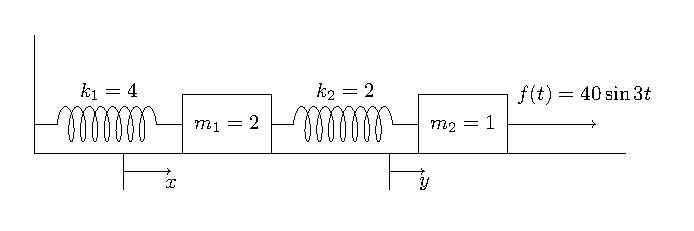
\includegraphics[scale=1.3]{Imagenes/sist_dos_masas.eps}
    \caption{Sistema masa-resorte que satisface el problema con valores iniciales.}
    \label{fig:figura_005}
\end{figure}
Escribiendo $X(s) = L \big[x(t)\big]$ y $Y(s) = L \big[y(t)\big]$, entonces las condiciones iniciales dadas en (\ref{eq:ecuacion_009}) implican que
\begin{align*}
L \big[\stilde{x} (t)\big] &= s^{2} \, X(s) \\[0.5em]
L \big[\stilde{y} (t)\big] &= s^{2} \, Y(s)
\end{align*}
Debido a que $L \big[\sin 3 \, t \big] = 3 / (s^{2} + 9)$, las transformadas de las ecuaciones dadas en (\ref{eq:ecuacion_008}) son las ecuaciones
\begin{align*}
2 \, s^{2} \, X(s) &= - 6 \, X(s) + 2 \, Y(s) \\[0.5em]
s^{2} \, Y(s) &= 2 \, X(s) - 2 \, Y(s) + \dfrac{120}{s^{2} + 9} 
\end{align*}
De esta manera, el sistema transformado es:
\begin{center}
\begin{tabular}{r r l}
$(s^{2} + 3) X(s)$ & $-Y(s)$ & $=0$ \\
$-2X(s)$ & $+(s^{2} + 2) Y(s)$ & $=\dfrac{120}{s^{2}+9}$ 
\end{tabular}
\end{center}
El determinante de este par de ecuaciones lineales en $X(s)$ y $Y(s)$ es
\begin{align*}
\mqty|
s^{2} + 3 & -1 \\
-2 & s^{2} + 2
|
 = (s^{2} + 3)(s^{2} + 2) - 2 = (s^{2} + 1) (s^{2} + 4 )
\end{align*}
y resolviendo el sistema dado, se tiene
\begin{align*}
X(s) = \dfrac{120}{(s^{2} + 1)(s^{2} + 4)(s^{2} + 9)} = \dfrac{5}{s^{2} + 1} - \dfrac{8}{s^{2} + 4} + \dfrac{18}{s^{2} + 9}
\end{align*}
y
\begin{align*}
Y(s) = \dfrac{120 (s^{2} + 3)}{(s^{2} + 1)(s^{2} + 4)(s^{2} + 9)} = \dfrac{10}{s^{2} + 1} + \dfrac{8}{s^{2} + 4} - \dfrac{18}{s^{2} + 9}
\end{align*}
La descomposición en fracciones parciales de las ecuaciones anteriores se encuentra fácilmente, ya que los factores del denominador son lineales en $s^{2}$, por lo que puede escribirse
\begin{align*}
\dfrac{120}{(s^{2} + 1)(s^{2} + 4)(s^{2} + 9)} = \dfrac{A}{s^{2} + 1} + \dfrac{B}{s^{2} + 4} - \dfrac{C}{s^{2} + 9}
\end{align*}
concluyendo que
\begin{align*}
120 =  A(s^{2} + 4)(s^{2} + 9) + B(s^{2} + 1)(s^{2} + 9) + C(s^{2} + 1)(s^{2} + 4)
\end{align*}
La sustitución de $s^{2} = -1$ (i.e. $s = i$ un cero del factor $s^{2} + 1$), en la ecuación anterior, hace que $120 = A \cdot 3 \cdot 8$, tal que $A = 5$. De manera similar, la sustitución de $s^{2} = -4$, nos proporciona $B = -8$, y de la sustitución de $s^{2} = -9$ se obtiene que $C = 3$.
\par
Las trasformadas inversas de Laplace de las expresiones anteriores, proporcionan la solución
\begin{align*}
x(t) &= 5 \, \sin t - 4 \, \sin 2 \, t + \sin 3 \, t \\[0.5em]
y(t) &= 10 \, \sin t + 4 \, \sin 2 \, t - 6 \, \sin 3 \, t
\end{align*}
El desplazamiento de las masas, se muestra en la siguiente figura:
\begin{figure}[H]
    \centering
    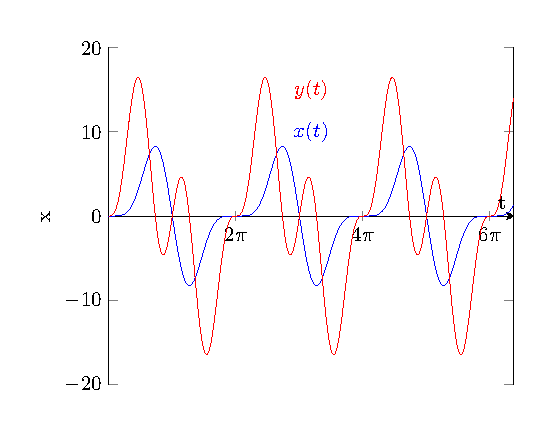
\includegraphics[scale=1.3]{Imagenes/sist_dos_masas_plot.eps}
    \caption{Funciones de la posición de $x(t)$ y $y(t)$.}
    \label{fig:figura_006}    
\end{figure}

\section{La perspectiva de la transformada.}

Considérese la ecuación general de segundo orden con coeficientes constantes como la ecuación de movimiento
\begin{align*}
m \, \stilde{x} + c \, \ptilde{x} + k \, x =  f(t)
\end{align*}
que corresponde a un sistema masa-resorte-amortiguador.
\begin{figure}[H]
    \centering
    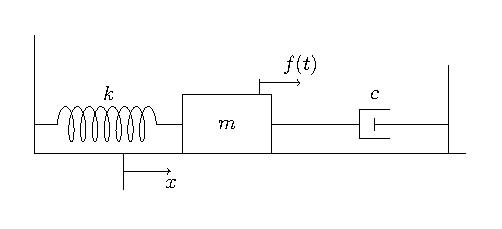
\includegraphics[scale=1.3]{Imagenes/sist_masa_resorte_dump.eps}
    \caption{Sistema masa-resorte-amortiguador con fuerza externa $f(t)$.}
    \label{fig:figura_007}
\end{figure}
Entonces la ecuación transformada es
\begin{align}
m \, \big[ s^{2} \, X(s) - s \, x(0) - \ptilde{x}(0) \big] + c \, \big[ s \, X(s) - x(0) \big] + k \, X(s) = F(s)
\label{eq:ecuacion_013}
\end{align}
Nótese que la ecuación (\ref{eq:ecuacion_013}) es una ecuación algebraica  - de hecho, una ecuación lineal - en la \enquote{incógnita} $X(s)$. Esta es la gran fuerza del método de la transformada de Laplace: \emph{Ecuaciones diferenciales se transforman en ecuaciones algebraicas fáciles de resolver}.
\par
Si se resuelve la ecuación (\ref{eq:ecuacion_013}) para $X(s)$, se obtiene:
\begin{align}
X(s) = \dfrac{F(s)}{Z(s)} + \dfrac{I(s)}{Z(s)}
\label{eq:ecuacion_014}
\end{align}
donde:
\begin{align*}
Z(s) = m \, s^{2} + c \, s + k \hspace{1cm} \mbox{ e }  I(s) = m \, x(0) \, s + m \, \ptilde{x} (0) + c \, x(0)
\end{align*}
Nótese que $Z(s)$ depende únicamente del sistema físico. Así, la ecuación (\ref{eq:ecuacion_014}) presenta $X(s)= L \big[x(t)\big]$ como la suma de un término dependiendo sólo de la fuerza externa y otro dependiendo sólo de las condiciones iniciales. En el caso de un sistema sin amortiguamiento, estos dos términos son las transformadas
\begin{align*}
L \big[x_{sp} (t)\big] = \dfrac{F(s)}{Z(s)} \hspace{1cm} \mbox{ y } L \big[x_{st} (t)\big] = \dfrac{I(s)}{Z(s)}
\end{align*}
de la solución periódica (sp) en estado permanente y de la solución transitoria (st), respectivamente. La única dificultad potencial en la búsqueda de estas soluciones se presenta al intentar obtener la transformada inversa de Laplace del lado derecho de la ecuación (\ref{eq:ecuacion_014}). 
\begin{teo}
Si $f(t)$ es una función continua por tramos para $t \geq 0$ y satisface la condición de orden exponencial $\abs{f(t)} \leq M \exp(c t)$ para $t \geq T $, entonces
\begin{align}
L \left[ \int_{0}^{t} f(t) \dd{\tau} \right] = \dfrac{1}{s} L \big[f(t) \big] = \dfrac{F(s)}{s}
\label{eq:ecuacion_017}
\end{align}
para $s > c$. En forma equivalente 
\begin{align}
L^{-1} \left[ \dfrac{F(s)}{s} \right] = \int_{0}^{t} f(\tau) \dd{\tau}
\label{eq:ecuacion_018}
\end{align}
\end{teo}
\begin{ejemplo}
Encuéntrese la transformada inversa de Laplace de
\begin{align*}
G(s) = \dfrac{1}{s^{2} (s - a)}
\end{align*}
En efecto, la ecuación (\ref{eq:ecuacion_018}) significa que se puede eliminar un factor de $s$ del denominador, encontrar la transformada inversa del resultado que se simplifica, y finalmente integrar de $0$ a $t$ (para \enquote{corregir} el factor $s$ faltante). Así se tiene que:
\begin{align*}
L^{-1} \bigg[ \dfrac{1}{s \, (s - a)} \bigg] = \int_{0}^{t} L^{-1} \bigg[\dfrac{1}{s - a} \bigg] \dd{\tau}  = \int_{0}^{t} \exp(a \, \tau) \dd{\tau} = \dfrac{1}{a} \, (\exp(a \, t) - 1)
\end{align*}
Repetimos la técnica para obtener
\begin{align*}
L^{-1} \bigg[\dfrac{1}{s^{2} \, (s - a)} \bigg] &= \int_{0}^{t} L^{-1} \bigg[\dfrac{1}{s(s-a)} \bigg] \dd{\tau} = \\[0.5em]
&= \int_{0}^{t} \dfrac{1}{a} \, (\exp(a \, \tau) - 1) \dd{\tau} = \\[0.5em]
&= \left[ \dfrac{1}{a} \, \left( \dfrac{1}{a} \, (\exp(a \, t) - \tau \right) \right] \eval_{0}^{t} = \\[0.5em]
&= \dfrac{1}{a^{2}} \, ( \exp(a \, t) - a \, t - 1)
\end{align*}
Esta técnica es con frecuencia más conveniente que el método de fracciones parciales para encontrar una transformada inversa de una fracción de la forma $\dfrac{P(s)}{(s^{n} \, Q(s))}$.
\end{ejemplo}

\begin{teo}
Si $F(s) = L \big[f(t)\big]$ existe para $s > c$, entonces  $L \big[\exp(a \, t) f(t)\big]$ existe para $s > a + c$ y
\begin{align*}
L \big[\exp(a \, t) \, f(t) \big] = F(s - a)
\end{align*}
De manera equivalente
\begin{align*}
L^{-1} \big[F(s - a)\big] = \exp(a \, t) \, f(t)
\end{align*}
Así la traslación $s \to s \to a$ en la transformada corresponde a la multiplicación de la función original de $t$ por $\exp(a \, t)$.
\end{teo}
Si se aplica el teorema de la traslación a las fórmulas de las transformadas de Laplace de $t^{n}$, $\cos k \, t$ y $\sen k \, t$ que ya se conocen  (multiplicando cada una de estas funciones por $\exp(a \, t)$ y reemplazando $s$ por $s - a$ en las transformadas) se obtienen lo siguiente:
\begin{align}
&{} f(t) \hspace{4cm} F(s) \nonumber \\[0.5em]
&{} \exp(a \, t) \, t^{n} \hspace{2cm} \dfrac{n!}{(s - a)^{n+1}} \hspace{0.5cm} (s > a)  \label{eq:ecuacion_106 } \\[0.5em]
&{} \exp(a \, t) \, \cos k \, t \hspace{1cm} \dfrac{s - a}{(s - a)^{2} + k^{2}} \hspace{0.5cm} (s > a)  \label{eq:ecuacion_107 }\\[0.5em]
&{} \exp(a \, t) \, \sin k \, t \hspace{1cm} \dfrac{k}{(s - a)^{2} + k^{2}} \hspace{0.5cm} (s > a)  \label{eq:ecuacion_108 }
\end{align}
\begin{ejemplo}
Considérese un sistema masa-resorte con $m = 1/2$, $k = 17$ y $c = 3$ en unidades mks. Como de costumbre, sea $x(t)$ la función que describe el desplazamiento de la masa $m$ a partir de su posición de equilibrio. Si la masa se pone en movimiento con $x(0)= 3$ y $\ptilde{x}(0) = 1$, encuentra $x(t)$ para las oscilaciones libres amortiguadas resultantes.
\begin{figure}[H]
    \centering
    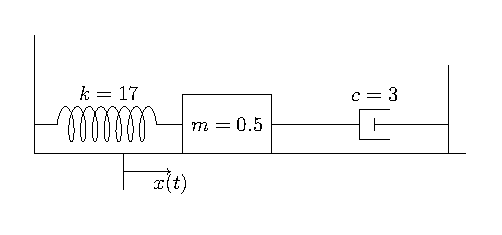
\includegraphics[scale=1.3]{Imagenes/sist_masa_resorte_dump_02.eps}
    \caption{Sistema masa-resorte-amortiguador.}
    \label{fig:figura_008}    
\end{figure}
La ecuación diferencial es:
\begin{align*}
\dfrac{1}{2} \, \stilde{x} + 3 \, \ptilde{x} + 17 \, x = 0
\end{align*}
de esta manera, debe de resolverse el problema con valores iniciales
\begin{align*}
\stilde{x} + 6 \, \ptilde{x} + 34 \, x = 0, \hspace{1cm} x(0) = 3, \hspace{0.3cm} \ptilde{x} (0) = 1
\end{align*}
Considérese la transformada de Laplace de cada término de la ecuación diferencial. Debido (obviamente) a que $L \big[0\big] = 0$, se obtiene la ecuación
\begin{align*}
\big[ s^{2} \, X(s) - 3 \, s - 1 \big] + 6 \, [s \, X(s) - 3 \big] + 34 \, X(s) = 0
\end{align*}
la cual se resuelve para $X(s)$ como 
\begin{align*}
X(s) = \dfrac{3 \, s + 19}{s^{2} + 6\, s + 34} =  3 \cdot \dfrac{s + 3}{(s + 3)^{2} + 25} + 2 \cdot \dfrac{5}{(s + 3)^{2} + 25}
\end{align*}
aplicando las fórmulas con $a = -3$ y $k = 5$, se observa que
\begin{align*}
x(t) = \exp(-3 \, t)(23 \, \cos 5 \, t + 2 \, \sin 5\, t)
\end{align*}
La figura (\ref{fig:figura_009}) muestra la gráfica de la oscilación amortiguada que decae rápidamente
\begin{figure}[H]
    \centering
    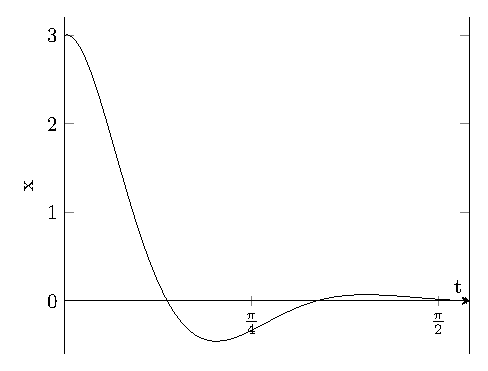
\includegraphics[scale=1.3]{Imagenes/sist_masa_resorte_dump_plot_02.eps}
    \caption{Sistema masa-resorte-amortiguador.}
    \label{fig:figura_009}
    \end{figure}
\end{ejemplo}
\begin{ejemplo}
Considérese el sistema masa-resorte-amortiguador del ejemplo anterio, pero con condiciones iniciales $x(0) = \ptilde{x}(0) = 0$ y con una fuerza externa aplicada $F(t) = 15 \, \sin 2 \, t$. Encuéntrense el movimiento transitorio resultante y el movimiento periódico en estado permanente de la masa.
\par
El problema con valores iniciales que se necesita resolver es
\begin{align*}
\stilde{x} + 6 \, \ptilde{x} + 34 \, x = 30 \, \sin 2 \, t, \hspace{1cm} x(0) = \ptilde{x}(0) = 0
\end{align*}
la ecuación transformada es:
\begin{align*}
s^{2} \, X(s) + 6 \, s \, X(s) + 34 \, X(s) = \dfrac{60}{s^{2} + 4}
\end{align*}
por lo tanto:
\begin{align*}
X(s) = \dfrac{60}{(s^{2} {+} 4) \, \big[(s {+} 3)^{2} {+} 25 \big]} = \dfrac{A \, s {+} B}{s^{2} {+} 4} + \dfrac{C \, s {+} D}{(s {+} 3)^{2} {+} 25}
\end{align*}
Cuando se multiplican ambos lados de esta ecuación por un denominador común, se tiene que:
\begin{align}
60 = (A \, s + B) \big[(s + 3)^{2} + 25\big] + (C \, s + D)(s^{2} + 4)
\label{eq:ecuacion_115}
\end{align}
Para encontrar $A$ y $B$ se sustituye el cero $s = 2 \, i$ del factor cuadrático $s^{2} + 4$ en la ecuación (\ref{eq:ecuacion_115}); el resultado es:
\begin{align*}
60 = (2 \, i \, A + B) \big[(2 \, i + 3)^{2} + 25 \big]
\end{align*}
el cual se simplifica en:
\begin{align*}
60 = (-24 \, A + 30 \, B) + (60 \, A + 12 \, B) \, i
\end{align*}
Ahora se igualan las partes reales e imaginarias de cada lado de esta ecuación para obtener dos ecuaciones lineales
\begin{align*}
-24 \, A + 30 \, B &= 60 \\[0.5em]
60 \, A + 12 \, B &= 0
\end{align*}
las cuales se resuelven para obtener que $A =- \dfrac{10}{29}$ y $B = \dfrac{50}{29}$.
\\[0.5em]
Para encontrar $C$ y $D$ se sustituye el cero $s = -3 + 5\, i$ del factor cuadrático $(s + 3)^{2}$ en la ecuación (\ref{eq:ecuacion_115}), y se obtiene:
\begin{align*}
60 = \big[C (- 3 + 5 \, i) + D\big] \, \big[(-3 + 5 \, i)^{2} + 4\big]
\end{align*}
que se simplifica en:
\begin{align*}
60 = (186 \, C - 12 \, D) + (30 \, C - 30 \, D) \, i
\end{align*}
Igualando las partes reales e imaginarias, una vez más se llega a dos ecuaciones lineales:
\begin{align*}
186 \, C - 12 \, D &= 60 \\[0.5em]
30 \, C - 30 \, D &= 0
\end{align*}
y se encuentra que su solución es $C = D = \dfrac{10}{29}$.
\par
Con estos valores de los coeficientes $A$, $B$, $C$, $D$, la descomposición en fracciones parciales de $X(s)$ es
\begin{align*}
X(s) &= \dfrac{1}{29} \, \left( \dfrac{-10 \, s + 50}{s^{2} + 4} + \dfrac{10 \, s + 10}{(s + 3)^{2} + 25} \right) = \\[0.5em]
&= \dfrac{1}{29} \, \left( \dfrac{-10 \, s + 25 \cdot 2}{s^{2} + 4} + \dfrac{10 (s + 3) - 4 \cdot 5}{(s + 3)^{2} + 25} \right)
\end{align*}
Después de calcular las trasnformadas inversas de Laplace se obtiene que la función de la posición es:
\begin{align*}
x(t) = \dfrac{5}{29} \, ( - 2 \, \cos 2 \, t  + 5  \, \sin 2 \, t ) + \dfrac{2}{29} \, (5 \, \cos 5 \, t - 2 \, \sin 5 \, t)
\end{align*}
En la gráfica (\ref{fig:figura_010}) se pueden ver las componentes periódica y transitoria, la suma de las dos, devuelve la posición $x(t)$ del sistema mecánico.
\begin{figure}[H]
    \centering
    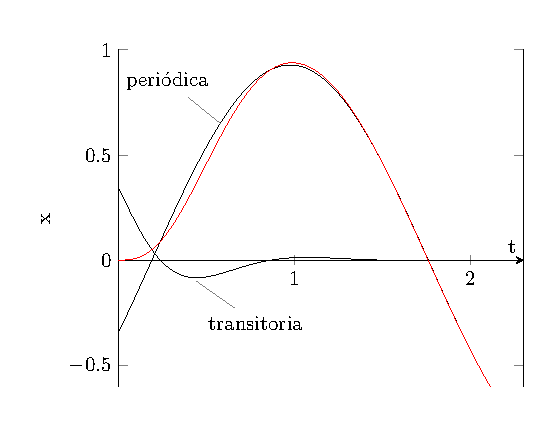
\includegraphics[scale=1.3]{Imagenes/sist_masa_resorte_dump_plot_03.eps}
    \caption{Oscilación periódica forzada $x_{sp}(t)$, movimiento transitorio amortiguado $x_{tr}(t)$ y solución $x(t) =x_{sp}(t) + x_{tr}(t)$.}
    \label{fig:figura_010}
\end{figure}
Los términos con frecuencia angular $2$ constituyen la oscilación forzada periódica en estado permanente de la masa, mientras que los términos exponenciales amortiguados con frecuencia angular $5$ constituyen su movimiento transitorio, el cual desaparece rápidamente, como se ve en la gráfica (\ref{fig:figura_010}). Nótese que el movimiento transitorio es diferente de cero aun cuando las condiciones iniciales sean cero.
\end{ejemplo}
\end{document}